\section{CNN optimizations on FPGA} \label{sec:opti_dataflow}
%
%
Section \ref{sec:fpga} provided a general layout of what is an \acrshort{fpga} and how did it work. This section is focused on how to implement a given model on an \acrshort{fpga}, and what hardware optimizations can be made to accelerate the inference.

Section \ref{sec:dt_general} reviews de various approaches to perform an efficient inference of a general \acrshort{cnn} on \acrshort{fpga}. 

Section \ref{subsec:impl_dsc} gives an overview of how to perform \acrshort{dsc} on \acrshort{fpga} and Section \ref{subsec:impl_prun} is focused on successful \acrshort{fpga}-based architecture that implemented pruning.
%
\subsection{General CNN inference on FPGA} \label{sec:dt_general}
%
As described in Section \ref{sec:fpga}, \acrshort{fpga} is an array of programmable gates that can interface with the outside world. As a result, to perform the convolution operation, the \acrshort{fpga} has to fetch weights and input \acrshort{fm} from the outside world (for example an external memory) and compute the convolution with them. Once the result is obtained, the \acrshort{fpga} can output the results through its \acrshort{ioe}.

According to \textcite{chen_eyeriss_2017}, the data movement can often be more energy-consuming than actual computation. Therefore, smart memory management is required to implement \acrshort{cnn} on low power devices such as \acrshort{fpga}. We discover in this section various techniques for handling the Datapath on the \acrshort{fpga}.

\subsubsection{Systolic Arrays}
%
%
Systolic arrays were implemented on the early \acrshort{fpga}-based accelerators \cite{abdelouahab_accelerating_2018, farabet_cnp_2009, gokhale_240_2014}. A static systolic array is a static array of \acrfull{pe}, controlled by the \acrshort{cpu}. The \acrshort{pe} is the basic computing unit for convolution. Therefore, each \acrshort{pe} is involved in a part of the computation and can communicate with adjacent \acrshort{pe}s. An illustration of this principle can be found in Figure \ref{fig:sytar}. The configuration can only support convolution with a kernel size $K_*$ lower than a maximal kernel size, such that $K_* \leq K_m$ (because the number of \acrshort{pe} is fixed). The systolic array allows spatial data reuse between rows and columns, high clock frequency, and temporal data reuse using \acrshort{fifo} queues \cite{joos_de_ter_beerst_accelerating_2019, mittal_survey_2020}.
%
\begin{figure}[H]
    \centering
    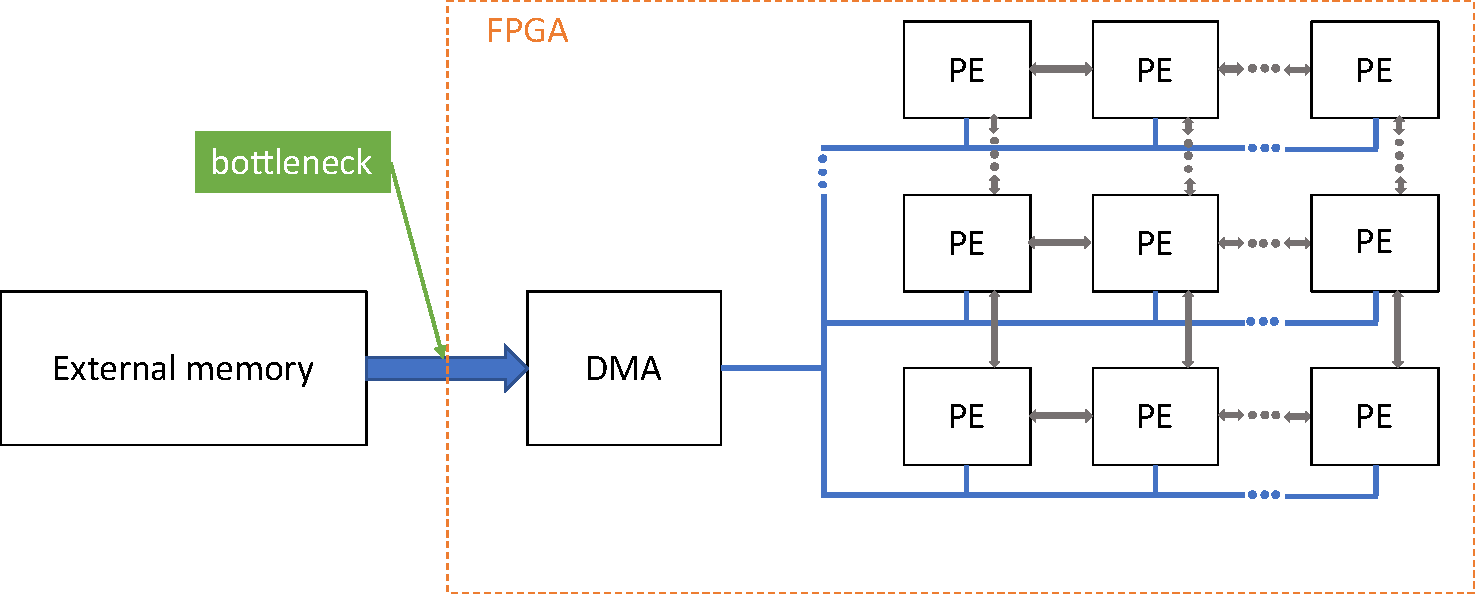
\includegraphics[width=\textwidth]{systArray.pdf}
    \caption{Static Systolic Arrays, inspired by \cite{abdelouahab_accelerating_2018}}
    \label{fig:sytar}
\end{figure}

However, Systolic Arrays have inefficiency problems. First, when the kernel size is much smaller than the maximal kernel size ($K_* << K_m$), there is an underutilization of the resources. For example, \cite{gokhale_240_2014} notes that for $3 \times 3$ kernels, only $9\%$ of the \acrfull{dsp} blocks are used. Second, data caching is not implemented. It means that it has always to fetch input from the external memory and it increases latency \cite{abdelouahab_accelerating_2018, wei_automated_2017}. The device performance is depending then on the memory bandwidth and it becomes memory-bounded. Furthermore, it is not energy efficient. According to \textcite{horowitz_11_2014}, the DRAM accesses severely impact both throughput and energy efficiency. External memory accesses are more expensive by several orders of magnitude in terms of energy and latency.
%
%
\subsubsection{Data-flow MoC for CNNs (2D mapping)}
%
%
Data-flow \acrfull{moc} can be used to accelerate \acrshort{cnn}s on \acrshort{fpga}. This approach is motivated by the feed-forward aspect of the inference stage of \acrshort{cnn}, which is purely data-driven \cite{abdelouahab_accelerating_2018}. Data-flow \acrfull{moc} was firstly investigated by \textcite{lin_li_low_2016}. \acrshort{cnn} can be represented as a graph where:
\begin{itemize}
    \item \textbf{Nodes} are processing units called \textit{actors}. Each actor follows a data-driven execution where the execution is triggered by the availability of input, which is the case for a \acrshort{cnn}.
    \item \textbf{Edges} are communication \acrshort{fifo} channels. Actors exchange data called \textit{tokens} through those \acrshort{fifo} channels.
\end{itemize}
A representation of such a network can be found in Figure \ref{fig:moc}, where $FM_{*}^{i}$ is the ith layer of the \acrshort{fm}.
%
\begin{figure}[H]
    \centering
    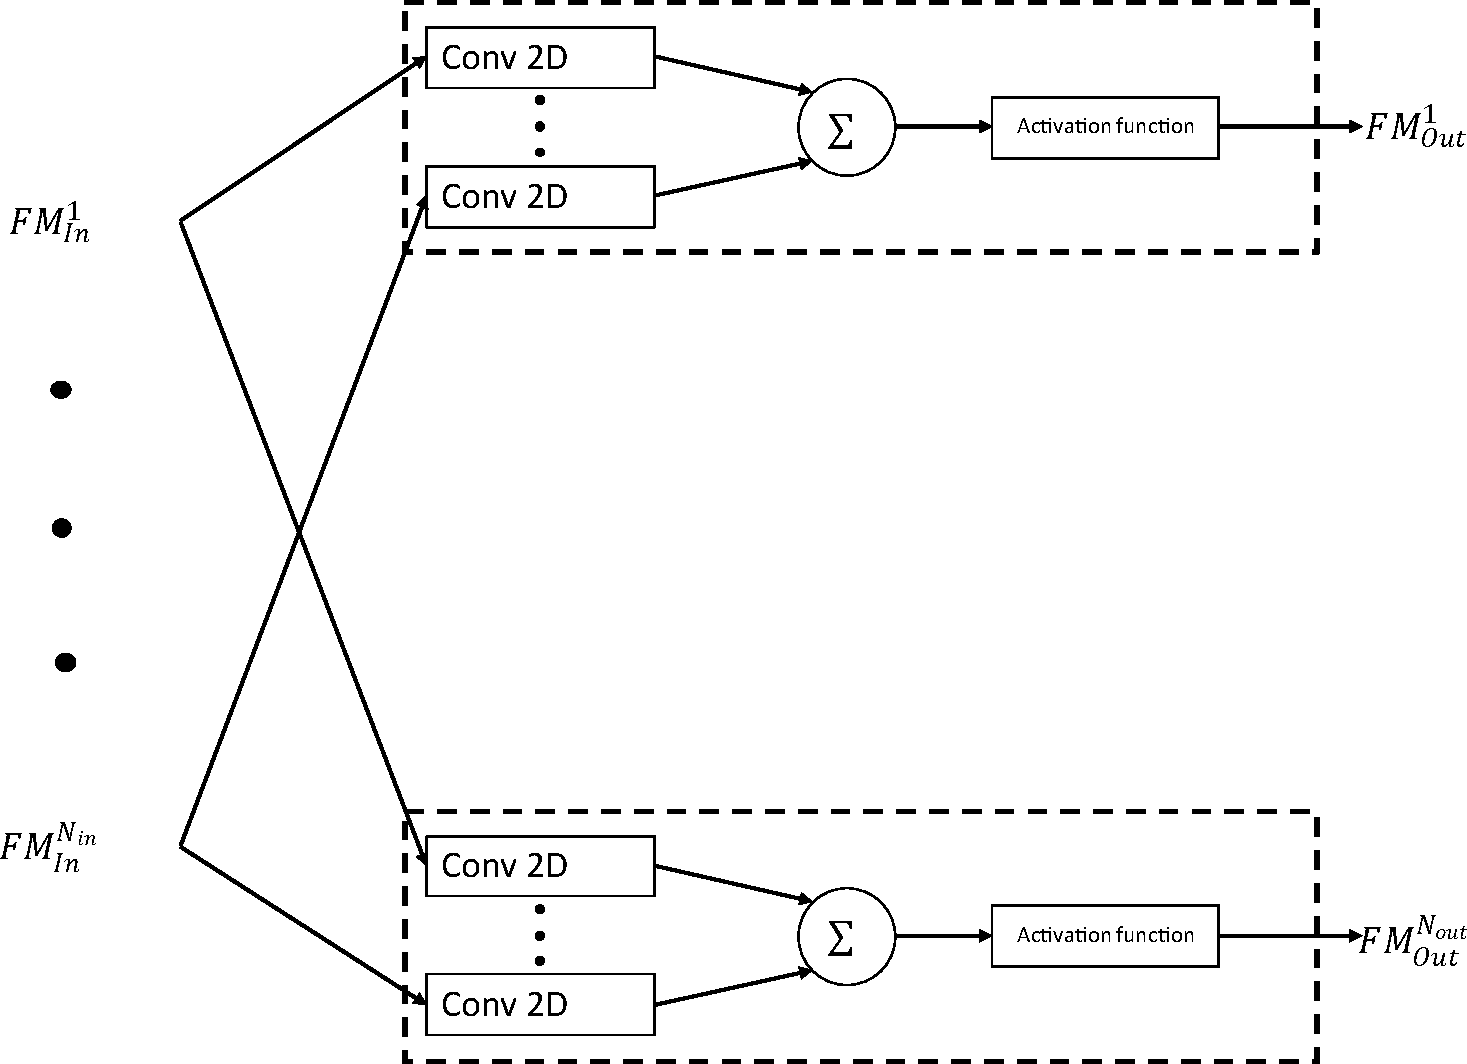
\includegraphics[width=0.6\textwidth]{Moc.pdf}
    \caption{Graph representation of a convolution layer, inspired by \cite{abdelouahab_accelerating_2018}}
    \label{fig:moc}
\end{figure}

As the number of tokens produced and consumed by an actor can be specified in a \acrshort{cnn}, we can apply a static data-flow \cite{lee_static_1987}. Therefore the \acrshort{cnn} can be modeled as a topology matrix and we only need to optimize those matrix components to minimize latency or energy consumption \cite{venieris_latency-driven_2017}. Those parameters are then used to derive \acrshort{pe} and buffer configurations. However, as pointed by \textcite{abdelouahab_tactics_2017}, we need to have direct hardware mapping between the graph and the \acrshort{fpga} to be efficient. It means that all the computations must be unrolled. However, we are then bounded by the hardware resources and the size of \acrshort{cnn}, preventing implementing this approach for deep models \cite{abdelouahab_accelerating_2018}.
%
\subsubsection{Loop Optimizations} \label{subsec:loopopti}
%
%
To overcome the inefficiencies of Systolic arrays and because Data-flow \acrshort{moc} can only be applied to small networks, data must first be cached into the on-chip memory of the \acrshort{fpga} before processing. However, according to \textcite{ma_optimizing_2018}, the on-chip memory of \acrshort{fpga} is not large enough to store all the data (requiring gigabytes). As a result, we need \textit{tiling} to fit a smaller portion of data into memory on-chip \cite{zhang_optimizing_2015}. We can summarize the dataflow as follow: the \acrshort{fpga} fetches a tile of data from external memory to on-chip buffers. Then the data is fed to the \acrshort{pe}s to compute the convolution. The results of the computation are transferred back to on-chip buffers and afterward, to the external memory. When the results are written back to memory, we can fetch a new tile of data. We can see the process in Figure \ref{fig:hierarchy}
%
\begin{figure}[H]
    \centering
    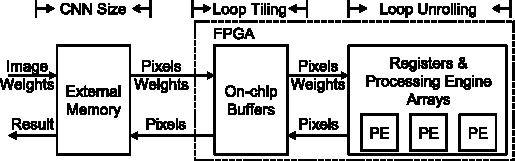
\includegraphics[width=0.75\textwidth]{memhiera.pdf}
    \caption{\acrshort{fpga} memory hierarchy, from \cite{ma_optimizing_2018}}
    \label{fig:hierarchy}
\end{figure}

Consequently, we can define a storage hierarchy with different energy costs. We can define the memory levels as \cite{sze_efficient_2017, horowitz_11_2014}:
%
\begin{enumerate}
    \item \textbf{External Memory}: it stores all the \acrshort{cnn} data. It has a large memory capacity (\textasciitilde GB) but accesses are costly in terms of energy and latency.
    \item \textbf{On-chip memory}: it stores the data fetched from external memory to feed the registers and \acrshort{pe}s. Accesses are less expensive to the external memory but it has less storage (\textasciitilde hundreds of KB).
    \item \textbf{Register}: is associated with the \acrshort{pe}s. The storage capacity is less than a few KB but it is faster and more energy-efficient. Accesses are 1 or 2 orders of magnitude lower energy than from External memory.
\end{enumerate}

Therefore, after tiling, the convolution operation can be decomposed in multiple loops, as observed in Figure \ref{fig:looptiling}. Nevertheless, an improper loop tiling may degrade the performance of the \acrshort{fpga} because we must minimize access to expensive memory levels. The major challenge when implementing a \acrshort{cnn} on \acrshort{fpga} is then to maximize data reuse in small cost memories. To address those problems, loop optimization techniques are applied to the nested loops in Figure \ref{fig:looptiling}. There are three techniques:
%
\begin{enumerate}
    \item \textbf{Loop tiling}: as said above, the on-chip memory of the \acrshort{fpga} is not large enough to store all the weights and \acrshort{fm}s of all \acrshort{cnn} layers \cite{abdelouahab_accelerating_2018}. The \acrshort{fpga} stores a tile of the data, accessed from the external memory, and the lower bound is set on the required on-chip buffer size. The tiling parameters represent the tile size. They are defined as $T_{*}$, where $*$ is the name of the dimension. For example, the size of an input pixel buffer (resp. output) is $T_{ix} \times T_{iy} \times T_{if} \times $ pixel\_datawith ( $ T_{ox} \times T_{oy} \times T_{of} \times $ pixel\_datawith). Furthermore, we have the following constraint: $T_{*} \leq N_{*}$.
    \item \textbf{Loop interchange}: it defines the order of sequential computation of the convolution loops. There are 2 types of loop interchange: \textit{intratile}, patterns of data movements from on-chip memory to registers (loop one to four in Figure \ref{fig:looptiling}); \textit{intertile}, patterns of data movements from external memory to on-chip buffers (the other loops).
    \item \textbf{Loop unrolling}: it determines the number of parallel computations. Four types of unrolling configuration can be done (depending on the loop to unroll). The different configurations can be seen in Figure \ref{fog:unroll}. As the \acrshort{fpga} has constrained resources, it is not always possible to fully unroll a loop. The unrolling parameters are defined as: $P_{*}$, where $*$ is the name of the dimension. We also have the following constraint: $P_{*} \leq T_{*} \leq N{*}$.
\end{enumerate}
%
\begin{figure}[H]
\centering
\begin{lstlisting}[language=Java]
for (int of=0;of<N;of+=Tof){
  for (int iy=0;iy<Niy,iy+=Tiy){
    for (int ix=0;ix<Nix,ix+=Tix){
      for (int if=0;n<C;if+=Tif){
        // DRAM: Load in on chip buffers the tiles
        // X[l,if:if+Tif,iy:iy+Ty,ix:ix+Tix]
        // Theta [l,n:n+Tof,if:if+Tif,j,k]
          for (int tof=0;tof<Tof;tof++){ -> Loop-4
            for (int tiy=0;tiy<Tiy,tiy++){ -> Loop-3
              for (int tix=0;tix<Tix,tix++){ -> Loop-3
                for (int tif=0;tof<Tif;tif++){ -> Loop-2
                  for (int ky=0;ky<Nky,ky++){ -> Loop-1
                    for (int kx=0;kx<Nkx,kx++){ -> Loop-1
                      Y[tof,tiy,tix] += X[tif,tiy+ky,tix+kx] *
                      W[tof,tif,ky,kx];
          }}}}}}
          // DRAM: Store output tile
}}}}
    \end{lstlisting}
    \caption{Loop Tiling, from \cite{abdelouahab_accelerating_2018}}
    \label{fig:looptiling}
\end{figure}
%
\begin{figure}[H]
    \centering
    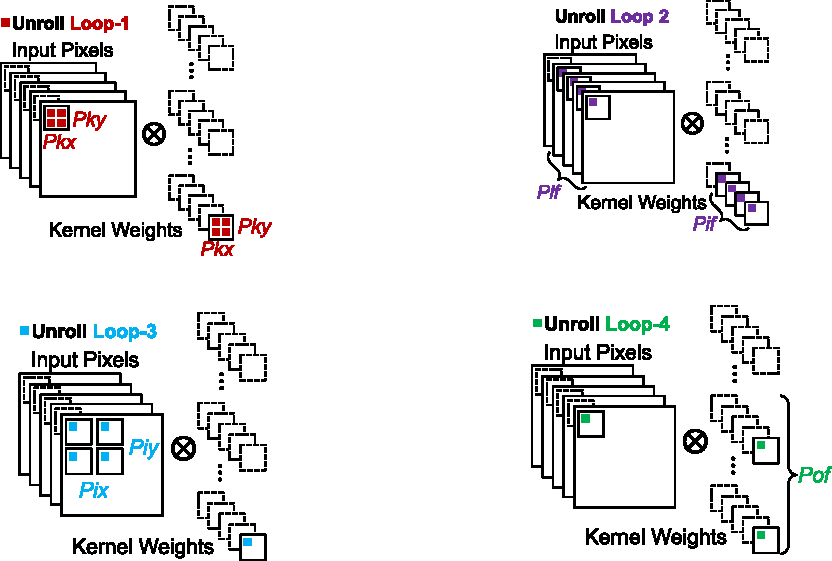
\includegraphics[width=\textwidth]{unroll.pdf}
    \caption{Loop unrolling configurations, from \cite{ma_optimizing_2018}}
    \label{fog:unroll}
\end{figure}

The loop optimization design variables determine the number of \acrshort{pe}s (unrolling parameters), the buffer size, and the number of external memory access (tiling parameters). We are going to review different studies of the design space exploration of unrolling parameters, tiling parameters, and loop interchange, to design the most efficient accelerator on the target platform.

The work of \textcite{zhang_optimizing_2015} proposes an analytical solution using the roofline model \cite{williams_roofline_2009} to identify the CNN design with the best performance and lowest \acrshort{fpga} resource requirement. They chose a loop unrolling of ($T_{if} \times T_{of}$) to avoid complex connection topologies for all arrays. It allows spatial reuse of pixels for $T_{of}$ unrolls, and the temporal reuse of weight for ($T_{ox} \times T_{oy}$). However, the disadvantage of this method is the need for a large local memory to store the partial sums ($T_{of} \times T_{ox} \times T_{oy}$).

Once the loop ordering and unrolling parameters have been set, the roofline model can be used to find the optimal tiling parameters. \textcite{mittal_survey_2020} defines this design space exploration method as: \textquote{\textit{The roofline model relates performance to computational performance and off-chip memory traffic}}. As an implementation can either be computation-bounded or memory-bounded, it uses those two limits to find the best trade-off between memory bandwidth and computational speed, where $CTC$ is the communication-to-communication ratio.
\begin{enumerate}
    \item \textbf{Computational roof}: $= \frac{\text{\# \ of \ operations}}{\# \ of \ execution \ cycles}$.
    \item \textbf{CTC ratio}: $= \frac{\text{\# \ of \ operations}}{\# \ of \ external \ data \ access}$
\end{enumerate}
Therefore, the achievable performance can be computed using equation \ref{eq:atperf}.
\begin{equation}
Att \ perf = min \ (Computational \ roof; CTC \ ratio \times bandwidth)
\label{eq:atperf}
\end{equation}

The roofline method is shown in Figure \ref{fig:roofmeth}. We can conclude that the best solution to pick is solution C since it offers the best performance while requiring the least bandwidth \cite{zhang_optimizing_2015}.
%
\begin{figure}[H]
    \centering
    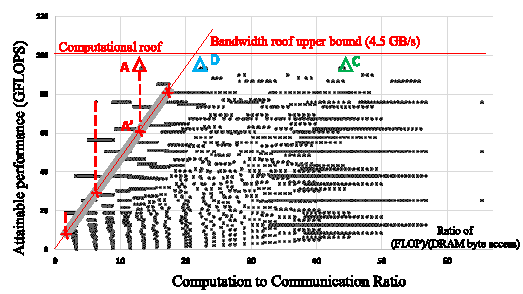
\includegraphics[width=\textwidth]{roofmethod.pdf}
    \caption{Design space of platform-supported designs, from \cite{zhang_optimizing_2015}}
    \label{fig:roofmeth}
\end{figure}

\textcite{motamedi_placid_2017} chose the best parameters according to the resources and the best data reuse scheme of the target platform. They did not tile on the kernel on the spatial axis because recent \acrshort{cnn}s have small filters and it would mean that a pixel can be loaded multiple times. As the tile goes over the input and output \acrshort{fm} channel, there is a choice between maximizing the reuse of the input \acrshort{fm} (MIR, each \acrshort{fm} is loaded once but some intermediate results have to be written back to memory) or output \acrshort{fm} (MOR, to avoid writing back intermediate results to memory but some input \acrshort{fm} have to be loaded more than once). Then they performed an exhaustive search on the tiling and \acrshort{pe} parameters to find the optimal design. It can be layer-specific (but the \acrshort{fpga} needs dynamic reconfiguration and \textcite{zhang_optimizing_2015} proved that it is inefficient) or values are fixed for all layers.

A different approach, studied by \textcite{ma_optimizing_2018}, proposes a design space exploration regarding various design objectives:
\begin{itemize}
    \item \textbf{Latency}: $P_*$ should be common factors of  $T_*$ for all convolution layers to fully utilize \acrshort{pe}s and $T_*$ should be the common factors of  $N_*$ to make full use of external memory transactions.
    \item \textbf{Partial sum storage}: to minimize the concurrent storage of partial sums in local memory and allowing to keep them into the PE, we should promote the computation of an output pixel to evacuate it to the external memory.
    \item \textbf{On-chip memory access}: on-chip memory access can be minimized by reusing at most pixels or weights in the \acrshort{pe}s.
    \item \textbf{External memory access}: to minimize external access, a sufficient buffer size should be assigned to pixels and weights.
\end{itemize}

They proposed two flowcharts in Figure \ref{fig:flowchart} to determine the number of partial sums and external accesses. 
%
\begin{figure}[H]
\centering
    \begin{subfigure}{.45\textwidth}
    \centering
    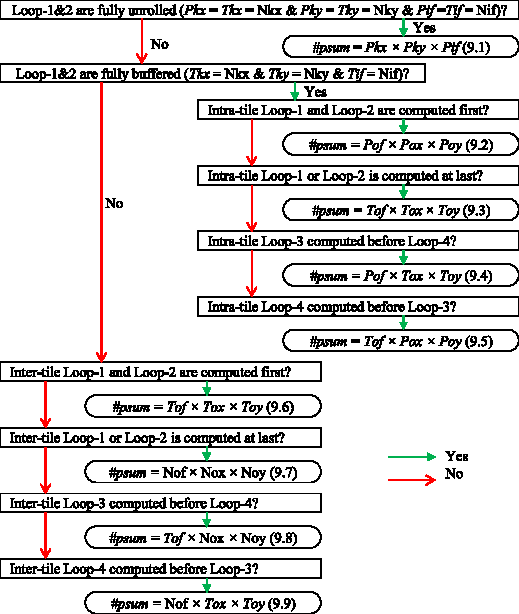
\includegraphics[width=\linewidth]{fwch1.pdf}
    \caption{ }
    \end{subfigure}
    \begin{subfigure}{.45\textwidth}
    \centering
    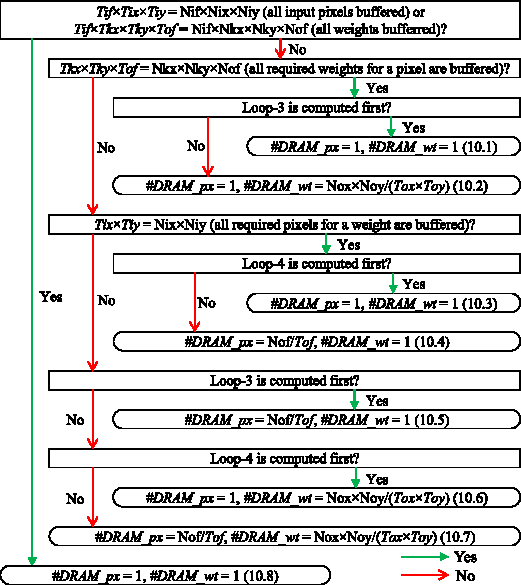
\includegraphics[width=\linewidth]{fwch2.pdf}
    \caption{ }
    \end{subfigure}
    \caption{Design space exploration of: (a) total number of partial sums that need to be stored in memory; (b) the number of external memory accesses, from \cite{ma_optimizing_2018}}
    \label{fig:flowchart}
\end{figure}

%
\subsection{DSC} \label{subsec:impl_dsc}
%
%
Some works put their interest in the implementation of the \acrshort{dsc}. In particular, we analyse the work of \textcite{bai_cnn_2018, liu_fpga-based_2019}. They present an \acrshort{fpga} accelerator that implement both standard and depthwise separable convolution. Networks like MobileNetV2 uses the 2 convolutions, the first one for not loosing to much information, the second one to speed up the inference. They both use a a commonly used \acrshort{dl} architecture that is called a heterogeneous system: a \acrshort{cpu} which controls the memory accesses and an accelerator that computes the convolution. The accelerator is designed in such a way that it can perform each layer of the network.

The accelerator in each work has the same structure. The accelerator uses weights, input and output buffers. To use the same accelerator for both convolutions, they firt compute an element-wise multiplication followed by an adder tree. The pattern of additions depens. \textcite{bai_cnn_2018} divides depthwise and pointwise convolution. As the element-wise multiplication produces a cuboid, we only have to sum either in the spatial or channel axis, either all the cuboid pixels to perform the desired convolution. On his side, \textcite{liu_fpga-based_2019} performs both convolution using the same adder tree. The dataflow to feed the adder tree depends then on the convolution. However, to use the same structure for both convolution, it pads some inputs with 0 value for separable convolution (the separable convolution has less arithmetic operations).

\begin{figure}
	\centering
	\includegraphics[width=\linewidth]{pingpong.pdf}
	\caption{Weight buffer in ping-pong structure, from \cite{bai_cnn_2018}}
	\label{fig:ping_pong_buffer}
\end{figure}
%
To improve the throughout of the network, they use a ping-pong buffer for the weight. Instead of using one buffer that stores the data for convolution, they use two buffers. Alternatively, one fetches weights for the next tile while the other is used for convolution. An illustration is found in Figure \ref{fig:ping_pong_buffer}.

Moreover, \textcite{liu_fpga-based_2019} has used the roofline model as method for design space exploration.
%
%
\subsection{Pruning} \label{subsec:impl_prun}
%
%
When implementing a pruned \acrshort{cnn} on an \acrshort{fpga}, we must address the problem of sparsity to keep the parallelism and the performance of the \acrshort{fpga} \cite{zhu_efficient_2020}. As a regular data access pattern is assured by applying a structured pruning scheme, there are some source of inefficiency that an implementation must handle.

First, the \acrshort{pe}s must avoid performing computation involving 0 weights. \textcite{kang_accelerator-aware_2020} fetches $N_{par}$ data in the channel axis and the $N_{non-zero}$ weights corresponding to the fetched group. A mutliplexer is used to choose the pixels associated to non-zero weights. An improvement can be made by avoiding 0 value pixel. \textcite{zhu_efficient_2020} clock gated the computation involving pixels with 0 value to save energy.

Second, in order to reduce the storage utilization, the zero-weights in a kernel must be discarded. The weights must be encoded in such a way that we keep both values and index of the weights to reduce the overhead of computing the output address.  Usually, kernels are encoded in format derived from the \acrfull{csr} \cite{mao_exploring_2017}. For example, \cite{zhu_efficient_2020} modified the format to compress further and accelerate the inference.

Finally, the problem of \textbf{load-imballance} can arise if the number of non-pruned weights is different in each \acrshort{pe} \cite{kim_zena_2018}. Therefore some \acrshort{pe} can finish before an other one and it can lead to inefficiency. \textcite{zhu_efficient_2020, kang_accelerator-aware_2020} solved this by setting an uniform number of weight in each kernels or group of fetched weights.

